%%%%%%%%%%%%%%%%%%%%%%%%%%%%%%%%%%%%%%%%%%%%%%
%% Modèle de rapport pédagogique v3.7
%%
%% Vincent Labatut 2014-2017
%%
%% v1     - 10/2014 : forme de rapport très différente
%% v2     - 02/2015 : modèle complètement refait
%% v2.1   - 03/2015 : définition de la page de titre
%% v2.2   - 03/2015 : correction de quelques bugs
%% v2.3   - 04/2015 : page de titre complétée (date, adresse postale, long titre)
%% v2.4   - 12/2015 : diverses modifications du contenu du document
%% v3     - 01/2016 : définition de la classe LaTeX, correction de quelques erreurs dans le texte
%% v3.1   - 02/2016 : package icomma pour les virgules décimales en français
%% v3.2   - 04/2016 : ajout de l'option "light" (pas de page de garde, compilation plus rapide)
%% v3.3   - 05/2016 : ajout de l'option "full" (page de garde, tables des figures et tableaux)
%% v3.4   - 10/2016 : un nom d'auteur par ligne, titre possible sur deux lignes
%% v3.5   - 09/2017 : ajout du pseudo-code (package algorithm2e) et du groupe en page de titre
%% v3.6   - 10/2017 : passage de la bibliographie en BibLaTeX (au lieu de BibTeX)
%% v3.7   - 11/2017 : paragraphes désormais plus numérotés, insertion optionnelle d'un résumé
%% v3.7.1 - 11/2017 : corrections diverses dans le contenu
%% v3.7.2 - 12/2017 : précision sur les références bibliographiques
%% v3.7.3 - 12/2017 : corrections diverses dans le contenu
%%
%% À faire :
%%  - mettre ToC dans bloc normal/light ? et que faire de ToF et ToT ?
%%  - fusionner modèles LIA/CERI ? (pb langue)
%%%%%%%%%%%%%%%%%%%%%%%%%%%%%%%%%%%%%%%%%%%%%%

% Le caractère '%' permet d'insérer des commentaires, qui seront
% ignorés par le compilateur.



%%%%%%%%%%%%%%%%%%%%%%%%%%%%%%%%%%%%%%%%%%%%%%%%%%%
%% Classe du document
%%%%%%%%%%%%%%%%%%%%%%%%%%%%%%%%%%%%%%%%%%%%%%%%%%%
% Classe utilisée sans option


\documentclass[light]{ceri}
\usepackage{graphicx}
\usepackage{titlesec}
\usepackage{listings}
\usepackage{pdfpages}
\usepackage{calc}
\usepackage[utf8]{inputenc}

\usepackage{color}
\usepackage{tikz}
\usetikzlibrary{shapes.geometric, arrows}
 
\definecolor{codegreen}{rgb}{0,0.6,0}
\definecolor{codegray}{rgb}{0.5,0.5,0.5}
\definecolor{codepurple}{rgb}{0.58,0,0.82}
\definecolor{backcolour}{rgb}{0.95,0.95,0.92}
 
\lstdefinestyle{mystyle}{
    backgroundcolor=\color{backcolour},   
    commentstyle=\color{codegreen},
    keywordstyle=\color{magenta},
    numberstyle=\tiny\color{codegray},
    stringstyle=\color{codepurple},
    basicstyle=\footnotesize,
    breakatwhitespace=false,         
    breaklines=true,                 
    captionpos=b,                    
    keepspaces=true,                 
    numbers=left,                    
    numbersep=5pt,                  
    showspaces=false,                
    showstringspaces=false,
    showtabs=false,                  
    tabsize=2
}
 
\lstset{style=mystyle}

% L'option "light" génère une version du document plus légère à compiler. 
% Elle est pratique lors de la phase de rédaction du document. Bien sûr, 
% la version finale du rapport, qui est rendue à l'évaluateur, ne doit 
% pas être compilée avec cette option.
%\documentclass[light]{ceri}

% L'option "full" rajoute une table des figures et une table des tableaux.
% À n'utiliser que pour de longs rapports contenant de nombreuses figures
% et/ou tableaux, ex. mémoire de M2. La page de titre apparaît.
%\documentclass[full]{ceri}


%%%%%%%%%%%%%%%%%%%%%%%%%%%%%%%%%%%%%%%%%%%%%%%%%%%
%% Informations générales
%%%%%%%%%%%%%%%%%%%%%%%%%%%%%%%%%%%%%%%%%%%%%%%%%%%
%TODO Titre du document, à adapter.
\title{Rapport Projet C/SD 2018}    

%TODO Liste des auteurs
\author{
  Rémy BANEL, \\
  Ali LABBAIZE , \\
  Paul-Louis FEULVARCH \\
} 


%TODO Groupe des auteurs
% Optionnel : seulement si le travail est réalisé en groupe (en l'absence de groupe, ne définissez pas la macro)
% Exemple : Groupe 1, G12, etc.
\groupe{Groupe de projet}

%TODO UE concernée par le rapport (à modifier).
% exemples : Projet Algorithmique
\classname{Nom de l'unité d'enseignement}

%TODO Formation concernée : à compléter.
% Exemples : Licence d'Informatique, Master d'Informatique.
\formation{Nom de la formation}

%TODO Parcours ou spécialité de la formation
% Exemples pour la licence : Systèmes et Réseaux Informatiques, Ingénierie Logicielle.
% Exemples pour le master : Ingénierie du Logiciel pour la Société Numérique, Réseaux Informatiques et Services Mobiles.
\parcours{Nom du parcours/spécialité}

% Désigne le fichier bibliographique à utiliser





% Il est possible de définir un résumé du document (optionnel) avec la commande \resume comme ci-dessous. 
% Si la commande n’apparaît pas, le résumé n'est pas inséré dans le document.
%\resume{Ce document est une introduction à \LaTeX{}. Il s'agit à la fois d'un tutoriel décrivant les principales fonctionnalités de ce système de composition de documents, et d'un modèle servant d'exemple à l'élaboration d'un document. Il utilise le fichier de mise en forme fourni pour l'écriture de rapports dans le cadre des enseignements donnés au CERI, Université d'Avignon.}
\begin{document}

%%%%%%%%%%%%%%%%%%%%%%%%%%%%%%%%%%%%%%%%%%%%%%%%%%%
% Page de garde
%%%%%%%%%%%%%%%%%%%%%%%%%%%%%%%%%%%%%%%%%%%%%%%%%%%

%%%%%%%%%%%%%%%%%%%%%%%%%%%%%%%%%%%%%%%%%%%%%%%%%%%
% Création de la page de titre.

\begin{center} 
        %
\includegraphics[width=0.7\textwidth]{images/Dasilflix.png}

\maketitle


\includegraphics[width=1.0\textwidth]{images/logos.png}
\end{center}

% pas de numérotation
\thispagestyle{empty}
% saut de page
\newpage
~
\thispagestyle{empty}
\newpage

\setcounter{page}{1}
\pagestyle{fancy}
%%%%%%%%%%%%%%%%%%%%%%%%%%%%%%%%%%%%%%%%%%%%%%%%%%%
%% Table des matiètes (template)
%%%%%%%%%%%%%%%%%%%%%%%%%%%%%%%%%%%%%%%%%%%%%%%%%%%
\MyToc

%%%%%%%%%%%%%%%%%%%%%%%%%%%%%%%%%%%%%%%%%%%%%%%%%%%
%% Corps du rapport
%%%%%%%%%%%%%%%%%%%%%%%%%%%%%%%%%%%%%%%%%%%%%%%%%%%
% La commande '\section' marque le début d'une nouvelle section.
% Elle prend le titre de la section en paramètre.
% Latex se charge d'effectuer la numérotation automatiquement.


%%%%%%%%%%%%%%%%%%%%%%%%%%%%%%%%%%%%%%%%%%%%%%%%%%%
%% Remerciements
%%%%%%%%%%%%%%%%%%%%%%%%%%%%%%%%%%%%%%%%%%%%%%%%%%%
% La commande '\section' marque le début d'une nouvelle section.
% Elle prend le titre de la section en paramètre.
% Latex se charge d'effectuer la numérotation automatiquement.
\section*{Remerciements}
%comme c'est une section un peu spéciale, on l'ajoute manuellement avec addcontentsline
\addcontentsline{toc}{section}{Remerciements}

Nous tenons à remercier MM.~DA SILVA et FESTOR pour leur disponibilité et leur écoute durant le projet, car certains points ont pu rapidement être éclaircis grâce à leur aide, et ce dans un court délai. \\

Les membres de l'équipe projet remercient également l'équipe pédagogique de TELECOM Nancy pour avoir donné aux élèves l'accès au MOOC gestion de projet de M.~Rémi BACHELET, ainsi que celui du GitLab de l'école, qui a permis un développement dans un grand confort, avec son interface agréable et ergonomique. \\

Pour finir, l'équipe souhaite remercier l'ensemble des encadrants du module C et SD pour le choix d'un sujet concret à la fois intéressant et formateur, autant dans le domaine de la programmation que de la gestion de projet, sans oublier l'ouverture au monde de la recherche scientifique.

%saut de page
\newpage

%%%%%%%%%%%%%%%%%%%%%%%%%%%%%%%%%%%%%%%%%%%%%%%%%%%
%% Introduction
%%%%%%%%%%%%%%%%%%%%%%%%%%%%%%%%%%%%%%%%%%%%%%%%%%%
\section{Introduction}
Les systèmes de recommandation sont de plus en plus rependus de nos jours sans même que nous nous en apercevions. De Youtube à Amazon, toutes les grandes entreprises se doivent de guider leurs utilisateurs. Ces algorithmes de recommandation sont primordiales pour l'économie de certaines entreprises car ils permettent à l'utilisateur de toujours trouver un objet à son goût et le poussent donc à consommer. On estime ainsi que 80\% des contenus visionnés sur le site de vidéos à la demande par abonnement Netflix le sont grâce à son système de recommandation. Ce nombre absolument gigantesque montre bien la nécessité qu'ont les entreprises d'essayer de rendre leurs algorithmes toujours plus performants, car ils peuvent être la clé de leur succès.\\
\indent L'amélioration de ces algorithmes passent inévitablement par les mathématiques. Les systèmes de recommandation forment donc un véritable objectif pour les chercheurs. Netflix a par exemple organisé un concours en 2006 afin que des gens proposent des améliorations pour son moteur de recommandation.\\
\indent Notre projet nous a donc amené à apporter notre patte dans ce vaste domaine des systèmes de recommandation en essayant de coder notre propre algorithme. Et cela s'avère ardu de transposer quelque chose qui parait simple pour un humain (nous pouvons tous facilement conseiller un ami sur un film car l'on connaît sans même s'en rendre compte ses goûts de manière assez précise) sous forme d'algorithme. Réussir à ce qu'une machine "devine" les goûts d'une personne en très peu de temps et quelques choses de plus complexe que l'on pourrait imaginer.  
%%Dans le domaine du traitement de l'information, la détection d'un objet spécifique au milieu d'autres du même type est un problème toujours d'actualité et amélioration constante avec la recherche qui y est menée. En effet, ces traitements ont de nombreuses utilités, que ce soit une chaîne de caractères dans un texte, ou bien un passage audio dans un échantillon sonore.\\

%Le projet du module Techniques et Outils pour la Programmation de cette année traite d'une application de ce domaine, à savoir la reconnaissance d'un motif dans une image par différentes approches : la recherche pixel par pixel, par histogrammes et par histogrammes intégraux. \\

%Notre équipe est constituée de deux anciens élèves de CPGE (MP), Ali LABBAIZE et Olivier GOUELLAIN et d'un ancien élève en DUT, Corentin SARDO. Ce dernier ayant le plus de connaissances remobilisables sur ce projet a été nommé chef de celui-ci. Cette diversité de formations d'origine a finalement abouti à une harmonie entre des talents complémentaires, pour finalement produire différents algorithmes ; mais aussi un état de l'art donnant une ouverture scientifique, ainsi que les éléments de gestion de projet et ce rapport. \\


\rule{8cm}{0cm}
\parbox{\linewidth-8cm}{\textit{\textbf {Nous vous souhaitons une bonne lecture. }}}
\newpage
%%%%%%%%%%%%%%%%%%%%%%%%%%%%%%%%%%%%%%%%%%%%%%%%%%%
%% Etat de l'art
%%%%%%%%%%%%%%%%%%%%%%%%%%%%%%%%%%%%%%%%%%%%%%%%%%%
\section{État de l’art}

Le premier algorithme de recommandation a vu le jour en 1992 avec Paul Resnick et John Riedl, deux chercheurs en informatique, qui ont proposé le premier système de recommandation, pour les articles d’Usenet\footnote[1]{Usenet est un système en réseau de forums, inventé en 1979. Pour fonctionner dans un environnement Unix, il utilise alors le protocole UUCP. Il devient accessible depuis Internet grâce à l'utilisation du protocole NNTP.}. Ce système collecte des notes données par les utilisateurs lorsqu’ils lisent des articles. Ces notes sont ensuite utilisées pour prédire à quel point les personnes n’ayant pas lu un article sont susceptibles de l’apprécier. Et ces prédictions sont basées sur le "filtrage collaboratif", dont le principe est simple: si une personne A a des idées similaires à une personne B sur certains sujets, alors il y a des chances que la personne A partage encore l'avis de la personne B sur un autre sujet, plutôt que celui d'une personne tirée au hasard.

Depuis, le sujet des systèmes de recommandation a pris beaucoup d'ampleur surtout avec toutes les applications qu'il a, sur des domaines assez sensibles, tels la politique et l'influence des choix des utilisateurs, avec la création des "bulles informationnelles". Des chercheurs tels que  P.~Resnick et J.~Riedl se sont intéressés à cette dernière, ce qui a donné naissance à des centaines d'algorithmes qui ont été utilisés pour l’implémentation de systèmes de recommandation. La plupart relève de concepts mathématiques avancés, qu'on peut classer selon 4 catégories.


\subsection{Approche 1 : Recommandation Personnalisée }
    Cette approche consiste tout simplement à proposer du contenu à l'utilisateur en se basant uniquement sur ses choix antérieurs, par le biais de listes prédéfinies de recommandations. On catégorise ainsi les utilisateurs de manière assez larges et peu précise, car le contenu n'est pas pris en compte dans l'équation.
    On retrouve cette approche avec certaines annonces publicitaires. Par exemple Adsense de Google est considéré comme un système de recommandation personnalisée qui se base sur le comportement passé de l’utilisateur (navigation, clics, historique de recherche,...)


\subsection{Approche 2 : Recommandation Objet (Content-Based filtering CB)\cite{Objet}}
    
    Une seconde approche serait donc d'accorder autant d'importance à l'objet qu'à la cible. Le système se baserait ainsi essentiellement sur les qualités et propriétés intrinsèques de l’objet lui-même tout en les corrélant avec les préférences et intérêts de l’utilisateur. On obtient donc un profil utilisateur (Figure \ref{profile_utilisateur}) ainsi qu'un profil objet. (Figure \ref{profile_livre})

    Une fois les profils créés\footnote[2]{ Il existe plusieurs façon de collecter les données nécessaires pour créer les profiles des utilisateurs ( filtrage actif, filtrage passif,... ) mais ceci ne fera pas l'objet de cet état de l'art. }, il est nécessaire d'évaluer à quel point un contenu pas encore vu par l’utilisateur est similaire aux contenus que celui-ci a évalués positivement dans le passé. Cette notion de similarité peut être mesurée de plusieurs façons:
        \begin{itemize}
            \item L'approche la plus simple est de ne prendre en compte qu'une seule valeur binaire. Par exemple, si le livre  se trouve dans la liste des genres préférés de l’utilisateur. Dans ce cas la similarité sera de 0 ou 1.
            
            \item Une approche plus sophistiquée consiste à s'intéresser à plusieurs données de l'objet (mots clés dans le cas des livres). Il suffit ensuite de mesurer quel objet est le plus proche des goûts de l'utilisateur. Pour cela, on peut par exemple utiliser le coefficient de Dice (donné par la formule $s=\frac{2|X \cap Y|}{|X|+|Y|}$ X et Y étant des ensembles finis quelconques).
        \end{itemize}
    
\begin{center}
\begin{figure}
    \centering
    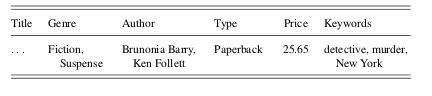
\includegraphics[width=0.7\textwidth]{images/profile_utilisateur.png} 
  \caption{Profile d'un utilisateur.}
    \label{profile_utilisateur}

\end{figure}   
\end{center}



\begin{center}
\begin{figure}
    \centering
    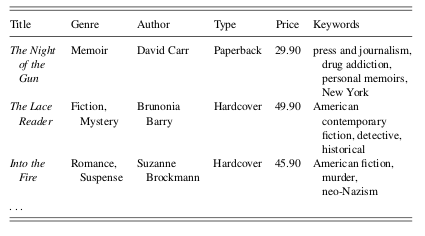
\includegraphics[width=0.7\textwidth]{images/profile_livres.png} 
  \caption{Profile d'un livre à recommander.}
    \label{profile_livre}

\end{figure}   
\end{center}


\subsection{Approche 3 : Recommandation Sociale\cite{social}}   
Ici, l'idée n'est plus de considérer un utilisateur unique, mais plutôt un ensemble d'utilisateurs. La recommandation se basant ainsi sur le comportement passé des utilisateurs similaires à l'utilisateur traité. On considère donc avec cette méthode que si deux individus ont présenté des intérêts similaires par le passé, alors ils partageront des goûts communs dans le futur.\\
 Ce type de recommandation se divise en 2 sous catégories:
    \begin{itemize}
        \item On peut traiter la recommandation du point de vue de l'utilisateur, cette méthode sera dite user-centric. On analyse quels utilisateurs présentent des intérêts communs afin de déterminer le voisinage proche de l'utilisateur traité. On se base sur ce voisinage et des objets qu'ils ont aimés afin de déterminer quel objet pourrait plaire à l'utilisateur analysé. Afin de déterminer à quel point deux utilisateurs peuvent être proches, on utilise généralement le coefficient de corrélation de Pearson qui se présente sous la forme \\
        {\Large $P_{a,u}=\frac{\sum_{i=1}^m (r_{a,i}-\bar{r_{a}}) \times (r_{u,i}-\bar{r_{u}}) }{\sqrt{\sum{i=1}^m (r_{a,i}-\bar{r_{a}})^2 \times \sum{i=1}^m (r_{u,i}-\bar{r_{u}})^2 }}$}  \\ 
        où:
            \begin{itemize}
                \item $a$ et $u$ sont des utilisateurs
                \item $r_{a,i}$ est la note donnée par l'utilisateur $a$ à l'objet $i$
                \item $\bar{r_{a}}$ est la moyenne des notes données par $a$
                \item $m$ est le nombre total d'objets
            \end{itemize}
        On prend ensuite les utilisateurs possédant le coefficient de corrélation le plus élevé avec l'utilisateur traité afin de créer son voisinage. Il ne reste plus qu'à calculer l'intérêt de l'utilisateur pour un objet donné à l'aide de la formule {\large$p_{a,i}=\bar{r_{a}}+\frac{\sum_{u=1}^n (r_{u,i}-\bar{r_{u}}) \times P_{a,u}}{\sum_{u=1}^n P_{a,u}}$} où:
            \begin{itemize}
                \item $p_{a,i}$ est la prédiction de l'objet $i$ pour l'utilisateur $a$ traité 
                \item $n$ est le nombre de personnes dans le voisinage de l'utilisateur $a$ traité
            \end{itemize}
        \item Mais on peut également utiliser le point de vue de l'objet, la méthode sera donc dite item-centric. L'idée est ici de mesurer la corrélation entre les objets à partir des notes attribuées par les utilisateurs. On Relis ainsi plusieurs objets entre eux et si l'utilisateur traité a aimé un objet donné, il lui sera conseillé un objet proche de celui en question.
    \end{itemize}
Cependant ce système présente un défaut majeur, il a besoin de nombreux utilisateurs pour être pertinent. Ainsi le lancement de tels systèmes souffre de l'absence d'utilisateurs afin d'obtenir des recommandations pertinentes.     

\subsection{Approche 4 : Recommandation Hybride}
Cette dernière approche des systèmes de recommandation consiste en un mélange des 3 précédentes. De plus, on va chercher à palier le cas où deux utilisateurs possédants les mêmes goûts n'ont pas évalué des objets en communs. Un filtrage par recommandation sociale (ou filtrage collaboratif) ne les considérera donc pas comme voisin et ne pourra donc pas se servir de leurs similarités afin de recommander un nouvel objet. Ici, l'idée sera donc d'assigner une valeur par défaut sur les objets notés seulement par l'un des deux utilisateurs. On améliore ainsi la prédiction en cas de rareté. Ce cas intervient lorsque la base de données du site est très grande par rapport au nombre d'utilisateurs. Dans ce cas, il est rare de trouver des utilisateurs ayant aimé les mêmes objets, la tâche de corrélation en devient très ardue. Ainsi lorsqu'un utilisateur n'a pas noté un objet, on va appliquer un filtrage item-centric, basé sur l'objet, afin de lui attribuer une pseudo note. Il sera donc plus facile de pouvoir comparer cet utilisateur à un autre à l'aide d'un filtrage user-centric. L'intérêt de ce système est de pouvoir compenser le lancement du système de recommandation. En effet, lors du lancement, il y a très peu d'utilisateurs et le filtrage collaboratif se retrouve fortement biaisé. Cette approche est de plus en plus utilisée et de grands groupes tels qu'Amazon et Netflix utilise une forme de celle-ci.

\subsection{Le cas Netflix}
Netflix est une entreprise américaine fondée en 1997. Elle propose aujourd'hui le visionnage de milliers de films et séries. Avec ses 125 millions d'abonnées, elle est aujourd'hui leader sur le secteur de la SVOD (la vidéo à la demande par abonnement). Cela est en grande partie dû à son algorithme de recommandation qui permet aux utilisateurs de rester sur la plateforme sans avoir besoin de chercher le contenu qui les intéresse. Ainsi, 80\% du contenu lu sur Netflix provient du système de recommandation, ce qui permet de rendre l'utilisateur passif, ce qui l'encourage à rester plus longtemps et à consommer du contenu.\\
\indent L'algorithme se base sur du machine learning en prenant en compte un certain nombre de paramètres:
\begin{itemize}
    \item la navigation de l'utilisateur sur la plateforme
    \item le temps de lecture d'une série, ceci dans le but d'en déterminer le niveau d'appréciation de l'utilisateur
    \item les séries que l'utilisateur a arrêté de regarder et au bout de combien de temps
    \item les séries que l'utilisateur a regardé précédemment
    \item l'heure à laquelle vous avez regardé telle ou telle série
    \item ce que l'utilisateur a regardé la semaine précédente, le mois précédent, voire l'année précédente la même époque
\end{itemize}
De plus, Netflix appose à chaque contenu différents "tags". Ceux-ci permettent de déterminer le "champ lexical" du contenu en permettant par exemple de savoir si la série se déroule dans le future, dans une grande ville, quels sont les personnages principaux (une femme, des enfants,...)\\
\indent Avec tout ceci, Netflix a établi 6 algorithmes principaux:
\begin{itemize}
    \item le Personalized Video Ranker qui propose pour chaque utilisateur un choix personnalisé en fonction des tags et de la popularité du contenu
    \item le Top-N Video Ranker qui fourni des recommandations pour chaque utilisateur en se basant uniquement sur les contenus les mieux classés par l'ensemble des utilisateurs
    \item l'algorithme de tendances récentes fonctionne comme le précédent mais en ne prenant en compte que les vidéos qui sont le mieux classés récemment, c'est-à-dire les tendance à court terme
    \item Le Continue Watching va lui se baser sur le contenu déjà visionné tout en corrélant notre point d'abandon d'une série
    \item l'algorithme de similitude vidéo à vidéo recommande un contenu en fonction de ce que l'on regarde actuellement. Cette algorithme est non personnalisé et se contente de renvoyer vers des vidéos prédéfinies similaires à celle que l'on regarde
\end{itemize}
Ceux-ci représentent les principaux algorithmes de recommandation de Netflix, mais ils ne sont pas seuls et c'est grâce à ces nombreux algorithmes faisant chacun des tâches précises que Netflix est parvenu à créer son système de recommandation. Celui-ci nécessite encore des améliorations bien évidemment. La société américaine souhaitant améliorer plusieurs points comme le fait de ne pas polluer nos recommandations avec une vidéo vue qui ne nous intéresse pas (par exemple des parents qui laissent leurs enfants regarder des vidéos). De même, Netflix souhaite améliorer la prédiction de l'évolution des goûts des enfants afin de toujours rester pertinent dans les choix de recommandation adressés aux enfants. 

\section{Choix de conception}
\subsection{Le Parsing}
Le parsing, ou extraction de données, est l'étape principale pour bien commencer le projet.
La première remarque qui peut être faite en lisant notre code de parsing \begin{math}foncion\_transfers.c \end{math}, est que celui-ci ne fait pas loin de 1000 lignes, ce qui est évidemment très long. Il nous semble donc important d'expliquer en détail les raisons de la longueur de ces fonctions de parsing.\\
\indent Tout d'abord il faut noter que toutes les recherches sont faites grâces à une seule fonction à savoir \begin{math} fgetc()\end{math}, un choix contraignant lorsque le code s'allonge, mais qui offre une sécurité contre les attaques passants par les fichers texte, comme cela a était présenté dans le TP de C sur le sujet. On évite ainsi l'utilisation de \begin{math} gets() \end{math} ou \begin{math} fscanf() \end{math} qui n'offrent pas de protection contre le buffer overflow\cite{bufferSecurity}. \\
\indent Certes le code s'en voit un peu rallongé, mais il en devient facilement compréhensible dans un même temps, dans le sens où toutes les fonctions de parsing  s'appuient sur le même principe de parcours caractère par caractère.  \\
\\

    \begin{lstlisting}[language=c]
    char *title (char* source, int id);
    char **actors (char* source, int id);
    char** tags (char* source,int id);
    int year ( char * source, int id);
    char * type(char * source, int id);
    char * director (char* source,int id) ;
    int duration (char* source, int id);
    \end{lstlisting}

    \begin{lstlisting}[language=c]
 		while (stock != EOF )
 			{
 				stock = fgetc(fichier);	
 				if (stock == 'W')
 				{
 					stock = fgetc(fichier);	
 					if (stock == 'i')
 					{
 						stock = fgetc(fichier);	
 						if (stock == 't')
 						{
 							stock = fgetc(fichier);
 							if (stock == 'h')
 							{
 								stock = fgetc(fichier);
 								stock = fgetc(fichier);
 								if (stock = ':')
 								{
 									break;
 								}
 							}
 						}
 					}
 				}
 			}
    \end{lstlisting}


\indent La récupération des tags (Comedy, Action ..etc) a posé quelques soucis, notamment pour récupérer le premier tag de chaque film. Nous nous sommes donc permis une seule modification du document fourni sur Arche \begin{math} BDCSD.txt \end{math}, à savoir l'ajout d'un " | " au début de la ligne contenant les tags et cela pour chaque film (Figure \ref{modif}), afin de faciliter l'accès à cette ligne.

\begin{center}
\begin{figure}[!h]

    \centering
    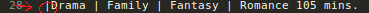
\includegraphics[width=0.7\textwidth]{images/modif.png} 
  \caption{Modification sur le fichier BDCSD.txt }
    \label{modif}

\end{figure}   
\end{center}

\indent Il faut également noter que nous avons travaillé sur 99 films et non pas 100, pour la bonne et simple raison que nous avons traité caractère par caractère, donc un nombre entre 10 et 99 représente le parcours de 2 caractères, un autre entre 100 et 999 représente le parcours de 3 caractères. Ajouter un traitement pour les id à 3 caractères pour un seul film ne nous semblait peu utile en début de projet lorsque d'autres tâches s'avéraient plus importantes. Cela ne rend pas pour autant notre code inadapté à une base de donnée plus large (à condition qu'elle respecte la même forme que celle qui nous a été fournis), il suffira de copier et ajouter une ligne pour chaque 0 qui s'ajoute à l'id (100, 1000 , 10000,... etc ).

    \begin{lstlisting}[language=c]
     	else if ((id < 100) && (id >= 10))
     		{
     		stock = fgetc(fichier);
    		while (stock != EOF) {
    			stock = fgetc(fichier);
    			if (stock == 48+(id/10)) {
    				stock = fgetc(fichier);
    				if (stock == 48 + (id%10)) {
    					stock = fgetc(fichier);					
    					if (stock == '.') {
    						break;
    					}
    				}
				}
		    }
    \end{lstlisting}


\subsection{Les calculs}
\subsubsection{Les structures de données utilisés}
    Avant de s'attaquer tête baissée dans les calculs, il fallait stocker toutes les données récupérées grâce au parsing. Nous avons dû allouer des espaces mémoire, qui dépendent de la nature du rendu de la fonction de parsing en question. Par exemple nous avons utilisé des tableaux de $char^*$ pour la fonction de récupération des tags ainsi que celle des acteurs.\\
    \indent Ensuite nous avons procédé à l'implémentations des dictionnaires (Hashmap). Ce choix de structure de données était motivé par plusieurs facteurs:
    \begin{itemize}
        \item Pouvoir associer à chaque id de film ($int$)
        une note ($float$), et les stocker ensemble.
        \item Pouvoir trier les résultats de recommandation en ordre décroissant suivant la note, mais que l'id du film reste liée au film (chose impossible à faire avec un tableau usuel).
        \item faciliter l'accès et la visualisation des données.
    \end{itemize}
    Les structures $Hashmap$ et $hashmap\_element$ sont toutes les deux implémentées avec les prototypes des foncions associés (nous avons défini le strict nécessaire de fonctions pour réaliser les tâches d'affichage, de stockage et  de tri avec cette structure) dans le fichier $fonction\_calcul.h$ comme toutes les autres structures du projet.
    \begin{lstlisting}[language=c]
        typedef struct _hashmap_element{
        	int key;
        	float value;
        } hashmap_element;
        typedef struct _hashmap_map{
        	int table_size;
        	int* actual_size;
        	hashmap_element *data;
         } hashmap_map;
         // CONSTRUCTEURS //
        hashmap_element* cst_hashmapelement(int key, int value);
        hashmap_map* cst_hashmap (int size);
        // FONCTIONS DE MANIPULATIONS DES HASHMAP //
        void hashmap_add(hashmap_map m, hashmap_element e);
        void hashmap_tostring(hashmap_map m);
        void trihashmapvalue (hashmap_map m);
    \end{lstlisting}
    \\
    \indent Ensuite nous avons implémenté une structure $Matrice$ afin de coder une approche collaborative, mais finalement le projet a pris une autre direction: nous avons fait le choix de présenter cette approche de manière théorique dans la rapport (explication: cf "points d'amélioration et suggestions").\\
    \begin{lstlisting}[language=c]
        typedef struct Matrice{
            int nbLigne;
            int nbColonne;
            float cases[nbLigne][nbColonne];
        }Matrice; 
    \end{lstlisting}
\subsubsection{calcul de la note}
    Une fois que nous avons défini toutes les structures de données, nous nous sommes attaqué aux structures $film$ et $utilisateur$ :
    \begin{lstlisting}[language=c]
        typedef struct Film{
        	int     id;
        	char    titre[400];
        	char    realisateur[100];
        	char    type[50];
        	int     annee;
        	int     duree;
        	char ** acteur;
        	char ** tags;
        }Film;

        typedef struct Utilisateur{
        	int     id;
        	Film    likedmovies[3];
        }Utilisateur;
    \end{lstlisting}
    Nous avons défini un modèle où l'utilisateur fait 3 choix parmi les films proposés, et, en fonction de ces choix, nous calculons les préférences de cet utilisateur. Nous comparons tous les films dans la base de données avec ces préférences, et les plus similaires auront les notes les plus élevées. On peut schématiser notre modèle ainsi (Figure \ref{calc}) : 
    
\begin{figure}[H]

    \centering
    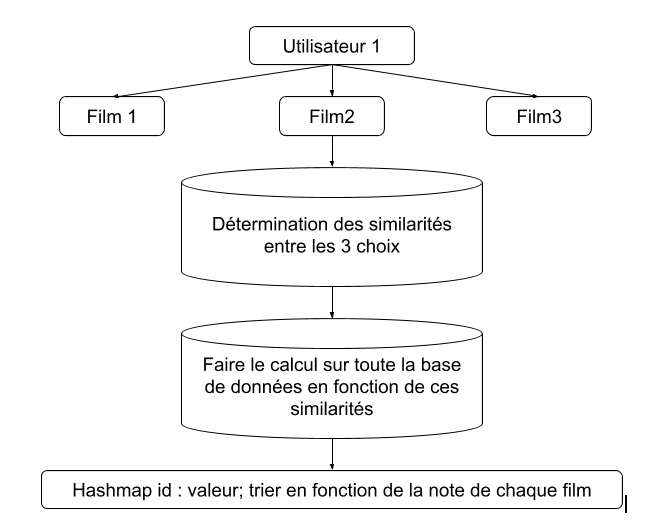
\includegraphics[width=0.8\textwidth]{images/calc.png} 
    \caption{Modèle de notre recommendation Objet }
    \label{calc}

\end{figure}   

    Le choix des films se fait au niveau de l'interface graphique. Il est envoyé aux fonctions de calcul, grâce à la fonction $Selection()$. Une fois les 3 id stockés, nous avons utilisé le principe de diviser pour régner\footnote[1]{Principe vu en TOP pendant le premier semestre, qui consiste à diviser : découper un problème initial en sous-problèmes. Puis régner : résoudre les sous-problèmes (récursivement ou directement s'ils sont assez petits). Pour finalement combiner : calculer une solution au problème initial à partir des solutions des sous-problèmes.}. Nous avons codé une fonction pour calculer la similarité entre les 3 films et cela pour chaque donnée à noter : 
     \begin{lstlisting}[language=c]
        int * favyear (Film f1 , Film f2 , Film f3);
        int * favduration (Film f1 , Film f2 , Film f3) ;
        int * favtags (Film f1 , Film f2 , Film f3);
        char * favrealisateur (Film f1 , Film f2 ,Film f3);
        char * favacteur (Film f1, Film f2, Film f3);
    \end{lstlisting}
    \begin{itemize}
        \item $favyear$: cette fonction prend l'année du film le plus récent et celui du plus ancien, et elle renvoie [ancien -4 , nouveau +4] afin de vérifier si le film à traiter est dans la même période cinématographique.
        \item $favduration$: même fonctionnement que $favyear$, avec un intervalle de -+15min.
        \item $favrealisateur$: cette fonction vérifie si un réalisateur est le même dans 2 des 3 films choisis, si oui elle le renvoie, afin de donner une note supplémentaire aux autres films de ce réalisateur.
        \item $favacteur$: elle fait l'intersection entre les acteurs des 3 choix, mais cette fois deux à deux, si un acteur se répère deux fois, on le garde, pour la même raison que le réalisateur.
        \item $favtags$: et finalement la fonction la plus importante (car on a fait le choix que la note attribuée aux genres soit la plus importante), cette fonction renvoie tous les tags qui se répètent au moins deux fois dans les tags des 3 films.
    \end{itemize}
    
\indent Une fois toutes les fonctions de calcul de similarités codées, il fallait les utiliser dans une grande fonction $calculnoteObjet$ qui prend en argument un profil de film et d'utilisateur, et renvoie la note qui représente le degré de similarité entre ce film et le profil de cette personne: 
     \begin{lstlisting}[language=c]
        float calculnoteObjet(Film f,Utilisateur u);
    \end{lstlisting}
Tout d'abord on initialise la note à 0, et ensuite, nous l'incrémentons suivant le système de notation suivant: 
    \begin{itemize}
        \item si le film est dans l'intervalle de $favyear$ --> 1.5
        \item si le film est dans l'intervalle de $favduration$ --> 0.5
        \item si le film a le même réalisateur que $favrealisateur$ --> 1.5
        \item si le film contient le même acteur que dans $favacteur$ --> 2.0
        \item et pour chaque tag similaire à un tag de $favtags$ --> 3.0/(le nombre de tags des films en question)
    \end{itemize}

Une fois la note attribuée au film, on la stock dans le hashmap avec les autres notes des autres films. Une fois que toute la base de donnée est parcourue, nous trions le hashmap et nous le renvoyons.\\
Finalement pour la fonction $tags$, afin de faciliter les calculs et les intersections des tableaux de tags, nous avons fait en sorte d'associer un tableau de 0 et de 1 à chaque film qui défini ses tags. Donc nous avons compté le nombre de tags totaux dans la base de données (on a créée un tableau de 18 cases, chaque case correspond à un tag, si le tag apparaît dans la description du film dans la case ça sera 1, sinon 0). Or ce choix contraint un peu le code. Lorsque nous incluons plus de films avec d'autres tags en dehors des 18 qu'on a déjà, cela oblige à l'ajouter dans la fonction $tagsbinaire$.
         \begin{lstlisting}[language=c]
                    
        int* tagsbinaire(Film f1){
        \* code raccourci pour comprendre le fonctionnement*/
        	int *tagsint = (int*) malloc(sizeof(int)*18);
        		if (strcmp(f1.tags[i], " Action " ) == 0{ 
        				tagsint[0]=1;	}
                    .
                    .
                    .
                    
        		else if (strcmp(f1.tags[i] , " Sport " ) == 0) {
        				tagsint[16]=1; }
        	}
        	return tagsint;
        }
    \end{lstlisting}


\subsection{L'interface graphique}
\subsubsection{La SDL}
\indent Nous avons choisi d'utiliser la bibliothèque SDL afin de réaliser l'interface graphique.Celle-ci est assez complète, elle permet de gérer le son, l'affichage d'un fenêtre et également de faire de la 2D. Elle est de plus libre de droit et gratuite, ce qui est un point non négligeable pour un projet tel que le notre. Nous avons rajouté 2 modules complémentaires pour faciliter certains redimensionnement d'images et d'affichage de texte. \\
\begin{table}[!h]

    \centering
    \begin{tabular}{|p{8cm}|p{8cm}|}
    \hline
        \rowcolor{yellow} Avantages  & Inconvénients   \tabularnewline \hline
        Rapidité à appréhender  & Difficulté d'apprentissage\tabularnewline \hline
        Facilité pour afficher des images (1 SDL\_Surface) &  Affichage dynamique\tabularnewline \hline
       Fonctions complémentaires &   Fonctions complémentaires\tabularnewline \hline
       Rapidité d'exécution  &   Utilisation d'images non compressées\tabularnewline \hline
  
        
    \end{tabular}
    \caption{Avantages et Inconvénients des fichiers de la SDL}
    \label{table1:SDL}
\end{table} \\


\indent La bibliothèque utilise des SDL\_Surface pour stocker un tableau de couleur qui correspond aux pixels des images chargées. Ainsi la fonction \begin{math}load\_image\end{math} permet de charger les images et de les associer aux surfaces de la bibliothèque SDL. Le programme renvoie un message d'erreur en cas d'échec de chargement, l'image n'existe pas ou ne comporte pas le nom émis par le programme. Une fonction \begin{math}apply\_surface\end{math} permet de simplifier l'affichage des images avec une position précise, au lieu de la fonction déjà implémentée à la bibliothèque SDL: \begin{math}SDLBlitSurface\end{math}. Il suffit de donner en argument les coordonnées (x,y) du premier pixel (situé en haut à gauche)(Figure \ref{coords1}), la SDL\_Surface où nous aurons charger l'image au préalable. Il faut également spécifier la Surface "de fond" qui sert de support à toutes les SDL\_Surface.\\
    \begin{lstlisting}[language=c]
    //Fonction pour bliter la surface //
    void apply_surface(int x, int y, SDL_Surface* source, SDL_Surface* destination){
        SDL_Rect offset;
    
        offset.x = x;
        offset.y = y;
    
        //Blittage de surface//
    SDL_BlitSurface(source,NULL,destination, &offset );
}
    \end{lstlisting}
    
\begin{figure}[!h]

    \centering
    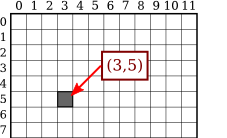
\includegraphics[width=0.4\textwidth]{images/coords1.png} 
  \caption{Système de coordonnées en SDL}
    \label{coords1}

\end{figure}   

\indent Au préalable, il faut initialiser SDL puis choisir le mode vidéo. Cela nous permet de spécifier les dimensions et les moteurs graphiques utilisés. Nous utilisons le moteur implémenté à la SDL: SDL\_HWSurface mais nous aurions pu également utiliser OpenGL (plus connu). Ce choix parait plus raisonnable, en effet, les problèmes de compatibilité sont moins fréquents car ce sont les mêmes développeurs qui ont élaboré la bibliothèque et le moteur graphique. Les dimensions retenues sont celle de la \begin{math}High\ Definition\ Standard\end{math}, ie 1280 par 720. Ainsi tous les écrans peuvent afficher notre programme de recommandation de films.\\
\indent La transparence est également gérée par la bibliothèque SDL, il faut spécifier la couleur qu'il faut "effacer" et rendre transparente.
    \begin{lstlisting}[language=c]
    //Rendre une couleur transparente//
    SDL_SetColorKey(logo, SDL_SRCCOLORKEY, SDL_MapRGB(logo->format, 255,255,255));
    \end{lstlisting}\\
\indent Pour actualiser la surface de "fond" et ainsi afficher les différentes images à l'écran, nous devons utiliser la fonction.\\ \begin{math}SDL\_Flip()\end{math}
    \begin{lstlisting}[language=c]
    SDL_Flip(ecran);
    \end{lstlisting}\\    

\subsubsection{Fonctionnement des pages}
\indent Chaque page est fonction de la précédente, le programme est donc relativement linéaire mais certaines fonctionnalités peuvent être amenées à se répéter et donc sont codées dans des fonctions pour éviter le code trop long. Ainsi la position de la souris, l'affichage d'images en cascade, avec des positions fixes ont été mises dans des fonctions. Également les différentes pages ont été codées dans des fonctions séparées pour faciliter la lecture et également la mémoire. En effet, nous pouvons vider la mémoire où sont stockées les images après avoir changé de page, il suffit de garder seulement les informations importantes (les numéros identifiant les films choisis, recommandés, position du curseur...).\\
\indent Afin de détecter toutes actions de l'utilisateur, nous avons créer des évènements, qui selon leur nature effectuent différentes tâches: renvoient à la page suivante, quittent l'application, affichent d'autres images... Une boucle while permet ainsi d'effectuer constamment une récupération du type d'évènement, qui est ensuite comparé selon l'action faite par l'utilisateur.\\
\indent Une difficulté a été de régler le passage de la souris (type d'évènement: SDL\_MOUSEMOTION) sur un bouton cliquable et de changer l'image en conséquence et de gérer la transparence de l'élément. Il faut réafficher alors toutes les images lorsque la souris n'est plus sur le bouton.\\
\indent La détection de l'action: cliquer sur un bouton, est détectée par l'évènement SDL\_MOUSEBUTTONUP. Ainsi le changement d'affichage s'effectue lorsque le bouton de la souris a été relâché, ce qui permet à l'utilisateur de relâcher le bouton de sa souris à une position différente du bouton, ainsi le changement d'affichage ne sera pas effectué.\\
\indent Afin de ne pas surcharger les capacités de l'ordinateur, on vide les images affichées sur la SDL\_Surface de "fond". Ainsi elles restent chargées mais ne surchargent pas l'interface et les graphismes de la machine.

\subsubsection{Fonctionnement des polices de texte}
\indent La bibliothèque SDL ne permet pas de traiter les affichages de texte, il faut installer un module supplémentaire: \begin{math}SDL\_ttf\end{math}. Ce module charge les polices de caractères présentes dans le dossier du programme. Ainsi les polices ont été choisies à l'avis du groupe. Nous pouvons également rajouter des types: souligné, gras, italique...avec le module chargé, une fois que ce dernier a été initialisé. \\
Plusieurs fonctions permettent d'afficher le texte dans le module. La fonction la plus puissante a été choisie. La transparence est totalement respectée avec l'image derrière, mais elle est légèrement plus lente à s'afficher. \\
\indent Les zones de texte fonctionnent de la même manière que les images: il est nécessaire de créer une SDL\_Surface pour libérer la mémoire disponible à l'affichage. Puis on "blitte" avec la fonction vue précédemment la surface avec le texte. On spécifie des positions pour fixer la surface. Puis on actualise la surface de "fond" pour que le texte apparaisse.\\
\subsubsection{La création des images}
Toutes les images ont été créées à l'aide du logiciel Gimp, qui a l'avantage par rapport à photoshop et illustrator d'être totalement gratuit. Évidemment la principale source d'inspiration des images a été les visuels de Netflix.\\


%%%%%%%%%%%%%%%%%%%%%%%%%%%%%%%%%%%%%%%%%%%%%%%%%%%
%% Résultats obtenus
%%%%%%%%%%%%%%%%%%%%%%%%%%%%%%%%%%%%%%%%%%%%%%%%%%%
\section{Résultats obtenus}

\subsection{Architecture et fonctionnement du projet}
    Concernant l'architecture adoptée pour ce projet (Figure \ref{archi}), nous avons réduit au maximum le nombre de fichier .c et.h que nous avons utilisé, un choix qui s'est avéré peu judicieux quand nous sommes arrivé à un stade avancé du projet.
    Nous avons quand même séparé le code en 3 grands fichiers:
    \begin{itemize}
        \item $fonction\_calcul.c$ qui contient tous les codes concernant le calcul des recommandations objets, et $fonction\_calcul.h$ qui contient toutes les structures précédemment illustrées (cf structures de données) 
        \item $fonction\_transfers.c$ pour les fonctions de parsing.
        \item Et finalement $interfacetest.c$ qui contient le main principal avec tout ce qui concerne l'interface graphique.
        \item 100 images en .bmp une pour chaque film, ainsi que les images qui ont servi de prototype, que nous n'avons pas réussi à mettre dans un seul fichier, parce que cela empêche l'automatisation de l'appel de ces derniers dans le code (notamment lors de la concaténation de caractères). 
    \end{itemize}
    
    \begin{figure}[!h]

        \centering
        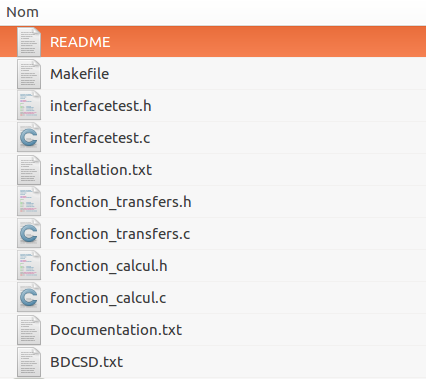
\includegraphics[width=0.4\textwidth]{images/archi.png} 
      \caption{Architecture du projet}
        \label{archi}

\end{figure}   

\subsection{L'impasse sur le stockage des résultats dans un fichier .json}
\indent L'approche du stockage des résultats dans un fichier spécifique .json n'a pu être abordée par le groupe en raison de l'avancée du projet. Nous n'avons pas pu enregistrer les données utilisateur et intégrer une interface utilisateur. Ainsi les données relatives à l'application ne sont pas sauvegardées lorsque l'application est quittée. Elles restent cependant stockées dans la mémoire vive lors de l'exécution du programme. L'approche utilisateur n'étant pas réalisée, le stockage de données est inutile dans notre cas.\\
\indent Cependant des recherches ont été faites sur les fichiers json, pour s'en servir éventuellement dans un futur projet où le stockage des résultats est inévitable. En effet, les json présentent un certain nombre d'avantages et d'inconvénients pour sauvegarder des données. 
\begin{table}[!h]

    \centering
    \begin{tabular}{|p{8cm}|p{8cm}|}
    \hline
        \rowcolor{yellow} Avantages  & Inconvénients   \tabularnewline \hline
       Format compatible par tous (humain \& machine)  & Garantir la sécurité des données \tabularnewline \hline
       Ne dépend d'aucun langage &  Syntaxe rudimentaire \tabularnewline \hline
       Permet de stocker des données de différents types  &   \tabularnewline \hline
  
        
    \end{tabular}
    \caption{Avantages et Inconvénients des fichiers .json}
    \label{table2:json}
\end{table} \\




	
\subsection{Exactitude des algorithmes}
  La seule exactitude que nous pouvons évaluer dans un projet de recommandation, c'est celle des calculs des préférences. Notre code de calcul (précédemment détaillé), et nous jugeons que les résultats renvoyés par notre algorithme sont potentiellement adaptés aux choix des utilisateurs, et quelques modifications ce sont faites au fur à mesure du projet, pour atteindre une précision plus fine.\\
  \indent Un exemple concret de ces modifications est le changement de la façon d'attribuer les notes en fonction des tags: nous avons remarqué que des films  apparaissent régulièrement dans les films recommandés par l'application, cela est dû au grand nombre de tags qui leur sont attribués dans le fichier .txt. naturellement ils vont contenir les tags préférés de l'utilisateur sans que le film soit vraiment totalement dans cette catégorie, donc nous avons dû diviser la note des tags par le nombres de ces derniers par film.
    
\section{Gestion de projet}  
\subsection{Priorisation des tâches}
Lorsque le projet a débuté, il était difficile de savoir dans quelle direction nous diriger. Il a donc fallut rapidement catégoriser les tâches principales en fonction de leur urgence et de leur importance pour le projet. C'est en cela que la matrice d'Einsenhower nous a été utile, pouvoir visualiser très rapidement ce qui serait primordial de faire et ce qui pouvait prendre un peu plus de temps à se mettre en route. Il nous a vite paru qu'une une bonne préparation du projet en amont serait inévitable afin de ne pas nous retrouver dépassés par les événements. Nous avons donc cherché à mettre l'accent sur la gestion de projet en début de celui-ci.



\begin{figure}[!h]
\centering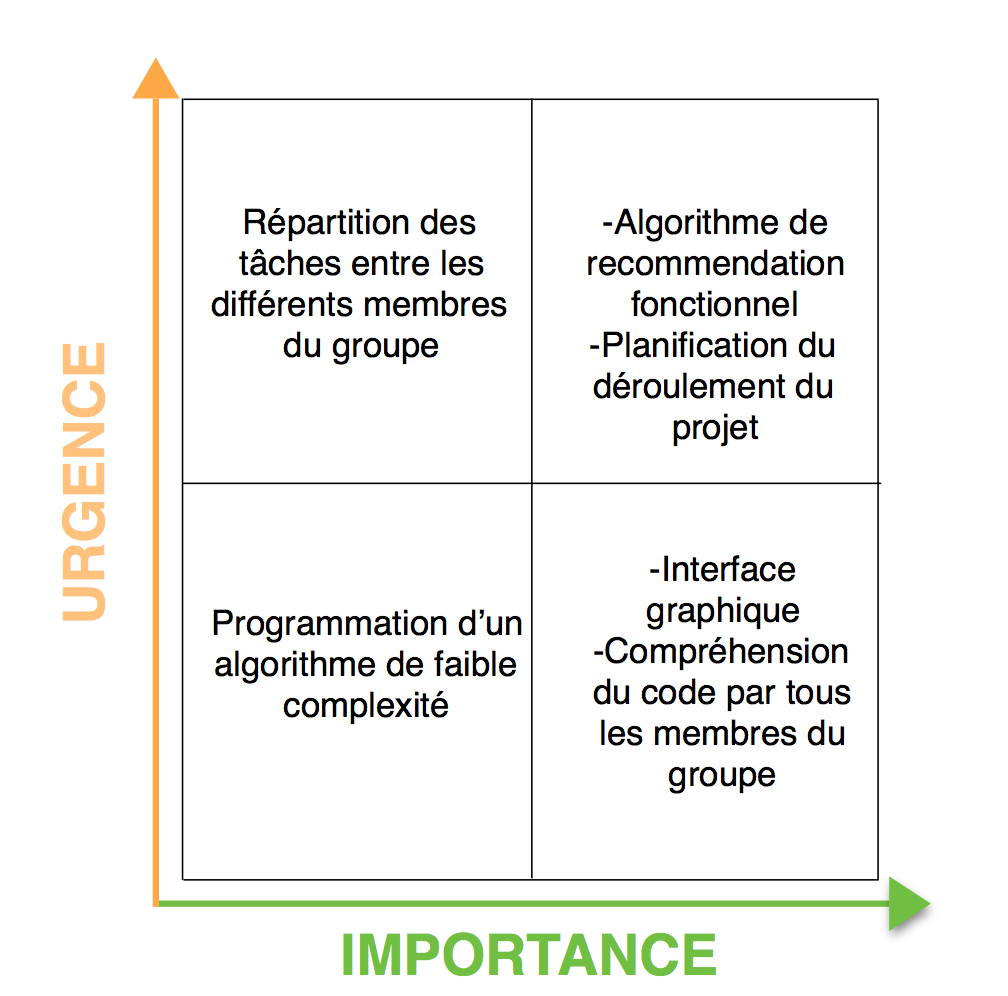
\includegraphics[width=13cm]{images/EISENHOWER.png}
\caption{Diagramme importance/urgence de notre projet}
\end{figure}
\newpage

\subsection{Répartition temporelle des tâches}
Une fois la priorisation des tâches effectuée, une tâche importante fût de jalonner le projet afin d'éviter de se retrouver pris par le temps. Dans ce but, le diagramme Gantt était l'outil qui nous semblait le plus adapté. Nous en avons donc réalisé un dès le début du projet, lorsque les principales étapes du projet ont été définies. Nous avons essayé de nous y tenir le plus possible, même si bien évidemment, divers imprévus font que les dates ne sont au final pas toujours respectées rigoureusement.

\begin{figure}[H]
\centering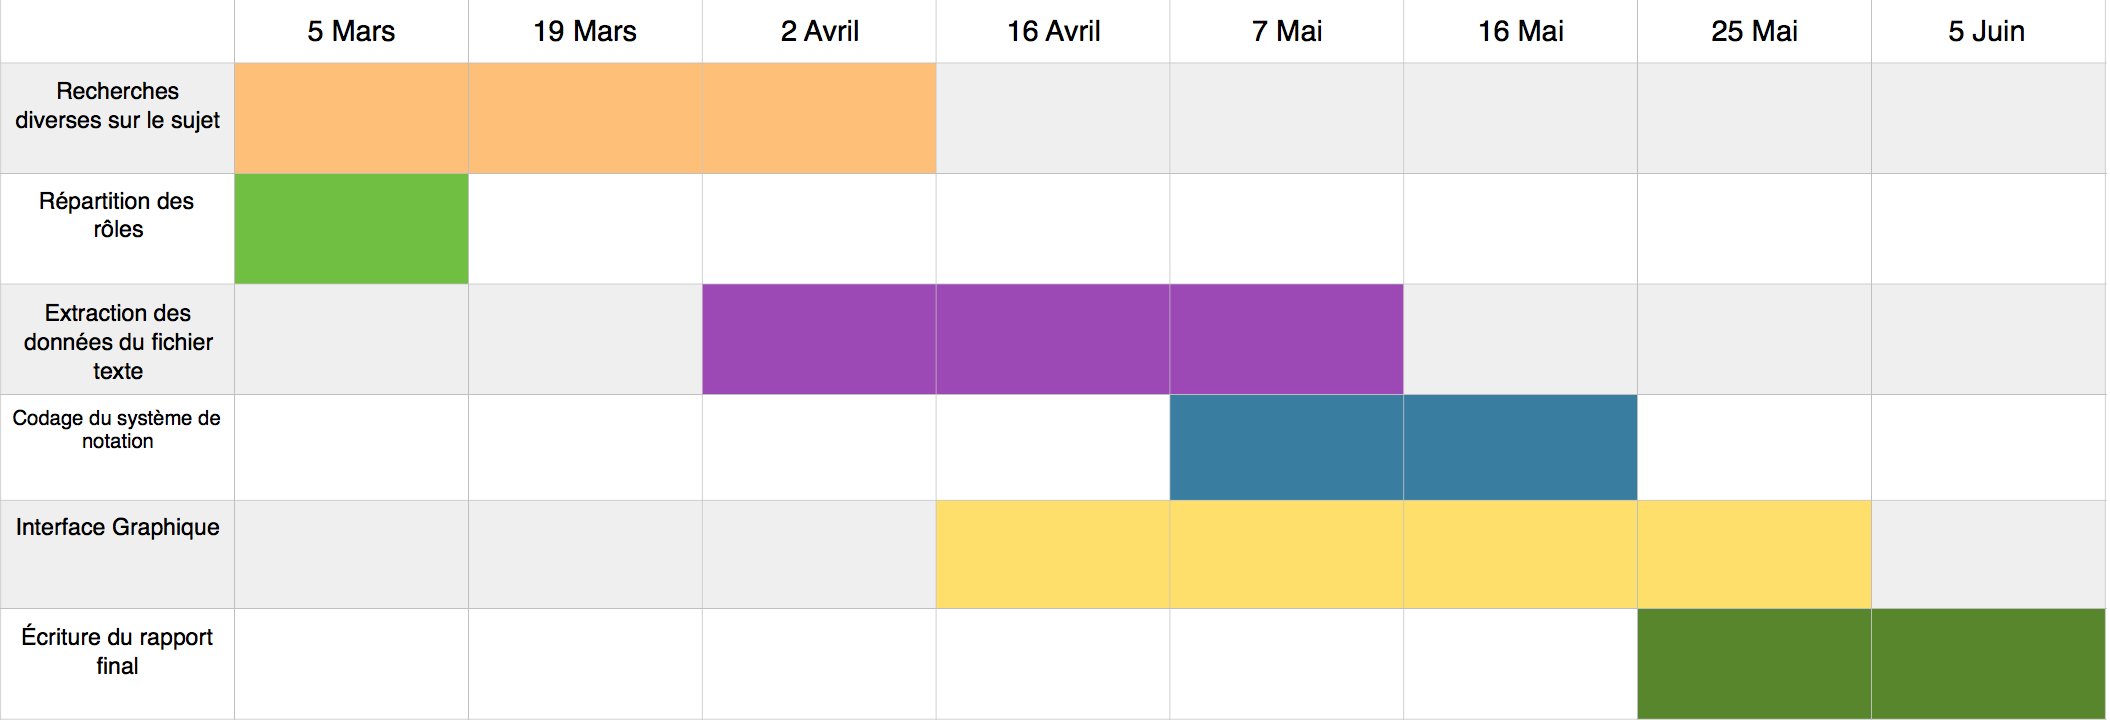
\includegraphics[width=17cm]{images/GANTT.png}
\caption{Diagramme prévisionnel des différentes tâches du projet}
\end{figure}  

Nous avons également réalisé, à titre d'indication, un second diagramme, réalisé une fois le projet fini. Celui-ci permet de voir les différences entre le gantt prévisionnel et ce qui a réellement été effectué.

\begin{figure}[H]
\centering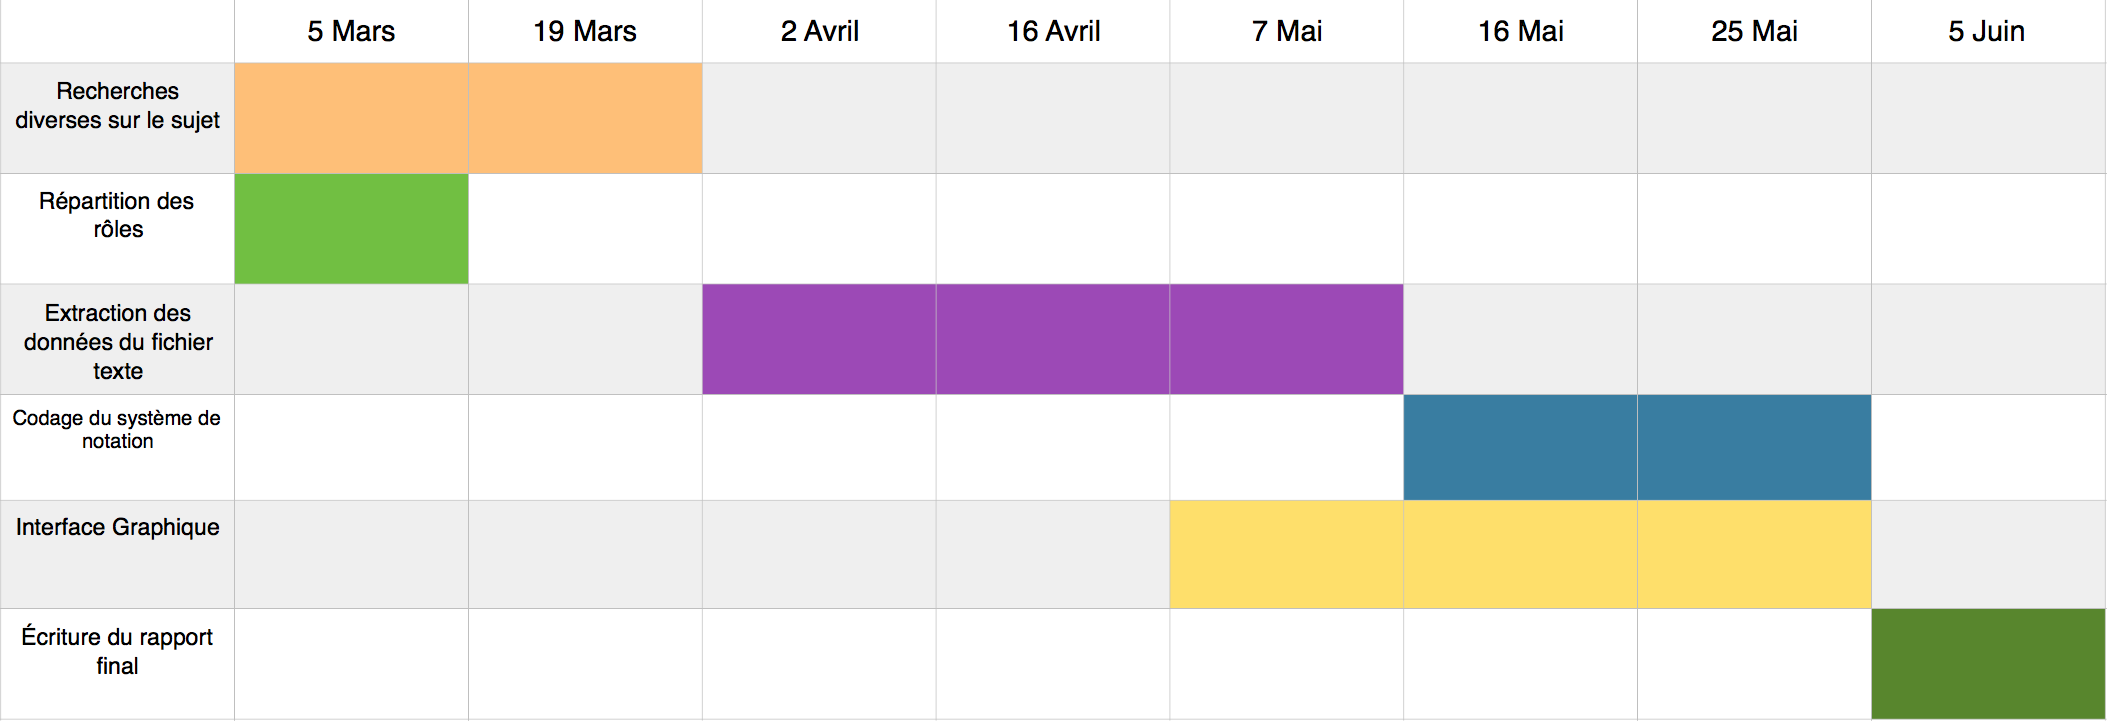
\includegraphics[width=17cm]{images/GanttFinal.png}
\caption{Diagramme final des différentes tâches du projet}
\end{figure} 

On constate que les différences sont plutôt minimes et n'ont pas dérangé outre mesure le déroulement du projet.

\subsection{Matrice SWOT}

La matrice SWOT est plus un outil de stratégie des entreprises, leur permettant
d’établir les menaces et les opportunités d’un nouveau produit. Dans notre cas, elle
nous a surtout permis d’établir une liste de nos faiblesses sur lesquelles nous devions
nous concentrer et nous améliorer afin de rendre le projet dans les meilleures conditions.

\begin{figure}[H]
\centering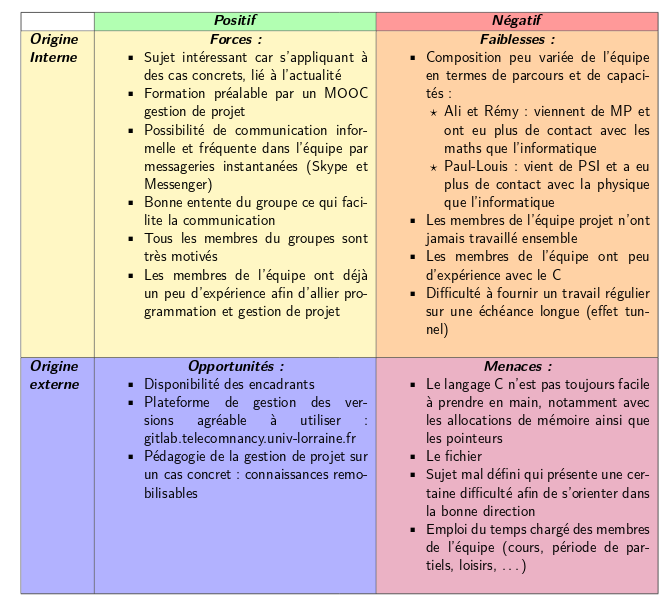
\includegraphics[width=18cm]{images/SWOT.png}
\caption{Diagramme prévisionnel des différentes tâches du projet}
\end{figure}  

\subsection{Matrice RACI}
Bien répartir les différentes tâches d'un projet est un élément essentiel afin de ne pas perdre de temps inutilement. En effet, si deux personnes se mettent à coder la même fonction, la perte de temps engendré sera non négligeable, d'où l'utilité de mettre en place une RACI très tôt afin d'éviter ce type de problème.

\begin{center}
\begin{tabular} {|c|c|c|c|}
\hline {}& {A.LABBAIZE} & {R.BANEL} & {PL.FEULVARCH} \\
\hline {Récupération des données du fichier texte} & {RA} & {I} & {R} \\
\hline {SDL} & {I} & {R} & {RA} \\
\hline {Système de recommandation} & {RA} & {CR} & {CI} \\
\hline {Création des images du jeu} & {CI} & {RA} & {I} \\
\hline {Fonctionnalités supplémentaires} & {RA} & {I} & {R} \\
\hline {Rédaction du compte rendu} & {RA} & {R} & {R} \\
\hline
\end{tabular}
\end{center}

\subsection{Comptes rendus}

Les différents comptes rendus de réunion on été placés en fin de rapport, dans la partie Annexes.

\section{Analyse post-mortem}


\subsection{Atteinte des objectif et efforts individuels réalisés}




Tout au long du projet, les tâches à effectuer ont été distribuées aux membres de l'équipe au fur et à mesure de l'avancement de celui-ci, selon les compétences de chacun, au cours des différentes réunions (Table \ref{table:efforts}).



\begin{table}[h]

    \centering
    \begin{tabular}{|p{4cm}|p{4cm}|p{4cm}|}
    \hline
        \rowcolor{yellow} Description  & Responsable  & Livrable \tabularnewline \hline
        Etat d'art & A.LABBAIZE & Fichier LaTex \tabularnewline \hline
        Se renseigner sur les interfaces graphiques & R. BANEL & - \tabularnewline \hline
        Réalisation du GANTT  & AL/PLF & Diagramme \tabularnewline \hline 
        Mise en forme de la matrice SWOT & R.~BANEL & Une matrice SWOT \tabularnewline \hline
        Algorithme de parsing des titres/années  & A.~LABBAIZE & Code C \tabularnewline \hline
        Algorithme de parsing des tags(genres)  & A.~LABBAIZE & Code C \tabularnewline \hline
         Algorithme de parsing des acteurs/réalisateurs  & A.~LABBAIZE & Code C \tabularnewline \hline
         Algorithme de parsing des durées  & A.~LABBAIZE & Code C \tabularnewline \hline
                Transformation des tags en données numériques afin de faciliter les calculs  & A.~LABBAIZE & Code C \tabularnewline \hline
         Création des structures film et utilisateur &  A.LABBAIZE & Code C\tabularnewline \hline

         
    \end{tabular}
    \caption{Analyse des efforts individuels}
    \label{table:efforts}
\end{table}


\begin{table}[H]

    \centering
    \begin{tabular}{|p{4cm}|p{4cm}|p{4cm}|}
    \hline   

       Rassembler les fonctions (fav) dans une seule fonction de calcul de recommandations et pondérer les résultats  & A.~LABBAIZE & Code C \tabularnewline \hline
       Implémentation de la structure Hashmap pour faciliter le tri et la visualisation des résultats  & A.~LABBAIZE & Code C \tabularnewline \hline

             Construire plusieurs fonctions (fav) qui calcule les préférences d'utilisateur, en se basant sur le choix de 3 films  & A.~LABBAIZE & Code C \tabularnewline \hline
         Modélisation théorique de l'approche sociale & A.~LABBAIZE & - \tabularnewline \hline
        Continuer l'état de l'art & R.~BANEL & Fichier LateX \tabularnewline \hline
        Coder une première interface graphique avec SDL & PLF & Code C \tabularnewline \hline 
        Coder un produit matriciel & R.~BANEL & Code C \tabularnewline \hline
        Coder un prototype de l'interface graphique & R.~BANEL & Code C \tabularnewline \hline 
        Visuels de l'interface graphique & R.~BANEL & Image .png \tabularnewline \hline 
        Récupérer les affiches des 99 films et séries de la liste & R.~BANEL & image \tabularnewline \hline
        Création du logo du programme  & R.~Banel & Image .png \tabularnewline \hline
        Implémentation de l'interface graphique  & PLF & Code C \tabularnewline \hline 
        Associer les fonctions de calcul et de parsing avec l'interface graphique  & A.LABBAIZE/PLF & Code C \tabularnewline \hline 
        Rédaction du rapport & Toute l'équipe &  Un Rapport LaTeX  \tabularnewline \hline
        
    \end{tabular}
    \caption{Analyse des efforts individuels}
    \label{table:efforts}
\end{table}

\subsection{Temps passé}
\begin{center}
\begin{tabular} {|c|c|c|c|}
\hline {}& {A.LABBAIZE} & {R.BANEL} & {PL.FEULVARCH} \\
\hline {La gestion de projet initiale} & {5h} & {3h} & {2h} \\
\hline {Recherches préliminaires} & {6h} & {4h} & {3h} \\
\hline {Extraction des données du fichier texte} & {48h} & {2h} & {-} \\
\hline {Système de notation} & {40h} & {2h} & {1h} \\
\hline {Conception des images} & {-} & {10h} & {-} \\
\hline {Interface graphique} & {5h} & {7h} & {55h} \\
\hline {Fonctions supplémentaires} & {10h} & {3h} & {-} \\
\hline {Tests divers} & {1h} & {2h} & {1h} \\
\hline {Rédaction du compte rendu} & {2h} & {10h} & {2h} \\
\hline {Total} & {117h} & {43h} & {64h} \\   
\hline
\end{tabular}
\end{center}


\subsection{Points positifs}
Les opportunités et forces mises en valeur dans la matrice SWOT réalisée au début du projet ont effectivement été saisies et exploitées : \\

\begin{itemize}
    \item La bonne entente entre les différents membres a permis une bonne communication au sein du groupe ce qui a été essentiel dans la répartition des tâches
    \item Le sujet intéressant a motivé l'équipe projet à s'investir pour voir aboutir les résultats
    
    \item La nécessité de réaliser une interface graphique a permis d'avoir une vision plus concrète du bon avancement du projet
    
    \item La formation préalable par un MOOC gestion de projet a permis de réaliser des documents ayant permis une meilleure organisation au cours du projet
    
    \item La communication par messagerie instantanée a été utile pour connaître l'avancement du projet quasiment en temps réel, tâche par tâche 
    
    
    \item Les encadrants ont pu éclaircir certaines interrogations sur le projet, cela nous a aidé à partir dans la bonne direction
    
    
\end{itemize}

%%%%%%%%%%%%%%%%%%%%%%%%%%%%%%%%%%%%%%%%%%%%%%%%%%%
\subsection{Difficultés rencontrées}
Même si nous avons tenté au maximum de réduire de façon pro-active les faiblesses et menaces mises en lumière dans la matrice SWOT, nous avons tout de même fait face à quelques une d'entre elles : \\

\begin{itemize}
    \item À cause de l'effet tunnel, il a été difficile de fournir un travail régulier sur une échéance longue, certaines périodes étant creuses en terme de travail fournis en comparaison avec d'autres périodes un peu plus "fasts"
    
    \item Le sujet qui n'était pas guidé (contrairement au sujet du premier semestre) a été un ralentisseur notable en début de projet. En effet, il était difficile au début de savoir dans quelle direction partir
    
    \item La recommandation sociale nécessitant la création d'une base de donnée d'utilisateurs n'a pu être mise en place
    
    \item Le stockage des données utilisateurs ainsi que l'implémentation d'une page d'inscription nous ont posé problème, ce qui nous a empêché de réaliser l'approche collaborative
    
    \item La réalisation de l'interface graphique s'est avérée déroutante au début car n'était pas vu en cours. Il a fallut de former de notre côté afin de pouvoir la réaliser\\
\end{itemize}

Au niveau du planning durant ce projet, la mise en place du travail a pris un certain temps. Les premières réunions étant là notamment pour essayer de voir quelle direction prendre pour bien début le projet. Ainsi les premières lignes de code ont mis du temps à voir le jour et nous avons dû attendre les vacances d'avril pour voir une avancée significative du projet. Cependant une fois le projet lancé, le travail a été assez régulier ce qui est un point plutôt positif.\\

Si on compare le temps prévu sur les tâches avec le temps passé, il est évident que de manière générale, les tâches ont mis plus de temps à être réalisées que prévu. Cela est dû à plusieurs facteurs. Certaines tâches semblaient abordables de prime à bord, mais se sont révélées plus ardues que prévu. On pense notamment à la fonction d'extraction des données du fichier texte qui nous été fourni. Un autre facteur de cette différence de temps était le soucis d'auto formation. Évidemment, nous n'avions pas toutes les connaissances requises en C pour un tel projet, notamment au niveau de l'interface graphique, il a donc été primordial de suivre plusieurs tutoriels afin de palier à ce problème, ce qui représente au final un temps assez important.


%%%%%%%%%%%%%%%%%%%%%%%%%%%%%%%%%%%%%%%%%%%%%%%%%%%
\subsection{Points d'amélioration et suggestions }

Au début du projet, le groupe envisageait un approche hybride, c'est-à- dire mélanger l'approche objet ( présenter dans le projet ), avec l'approche sociale qui se base sur le recyclage des données enregistrées de chaque utilisateur. Ainsi la recommandation est plus personnalisée (cf état de l'art). Une modélisation théorique est réalisée ainsi qu'une implémentation des structures nécessaires pour réaliser cette approche. Malheureusement une fois que le groupe a affronté la difficulté de l'implémentation de l'interface graphique en C, on a fait le choix de se restreindre à une seule approche fonctionnelle\footnote[1]{<<Commencez simple, et puis on verra ..>> - Sébastien Da-Silva} ( recommandation objet ).\\

Notre modélisation de cette approche se base essentiellement sur les matrices, et le stockage des films aimé par l'utilisateur dans un fichier txt. Par exemple pour un utilisateur non inscrit à notre logiciel, nous lui créeons un profil ( pseudo, mot de passe, id ...etc ), et nous enregistrons  toutes ses données dans le fichier \begin{math}id.txt\end{math}. Une fois tout cela est fait, pour la prochaine connexion d'un utilisateur (id = 1 par exemple), on récupère les 3 films les mieux noté par ce dernier, depuis ce fichier \begin{math}1.txt\end{math} dans ce cas, on applique la fonction \begin{math}calculnoteObjet;\end{math} entre ces 3 films et tous les autres films pour stocker chaque note résulante dans une matrice {\large$(U)_{0<i<100,0<j<100}$}, liée à chaque élément {$u_{i,j}$} soit à 1 ou à 0, en fonction de si la fonction renvoie une note de plus de 6/10 au film de id i*j on aura {$u_{i,j}=1$} sinon {$u_{i,j}=0$}. Une fois deux matrices de deux utilisateurs sont calculées nous avons décidé d'utiliser la norme 1 {\large$$||M||_1 = \sum_{k=0}^{n}|m_{ij}| $$} pour calculer la distance {\large$ d(U1,U2) = ||U1-U2||$} entre deux utilisateurs U1 et U2.\\
\\
\indent{\Large Illustration : }\\
\\
 \indent Soit {$U1$} et {$U2$} deux matrices de {$({\cal M})_{100}(R)$} définies ainsi : 
$$u_{i,j}=\left\lbrace
\begin{array}{ll}
0  &  \mbox{si calculnoteObjet(film(i*j),u) < 6}\\
1 &  \mbox{sinon}
\end{array}
\right.$$ 

Donc $U1$ ou $U2$ ressemblerons à : 
$$ \left\( 
\begin{array}{cccc}
0 & 1 &  \cdots & 0 \\
\vdots  & \ddots & \ddots & \vdots \\
1 & 0 &\cdots & 1
\end{array}\right\) $$

Une fois que la soustraction $U1 - U2$ est faite, plus les matrices sont similaires, plus de 0 seront présents dans la matrice résultante, donc la norme de cette soustraction (distance) sera petite, et vice versa.\\
\\
\indent L'idée était de calculer la distance entre les utilisateurs déjà inscrits chez nous, et si l'un d'eux désire une recommandation, on lui proposera un film aimé par l'utilisateur le plus proche de ce dernier, dans le sens de la distance précédemment définie. La structure matrice étant déjà définie, ainsi que la modélisation des calculs, le problème restait dans l'implantation d'une page d'inscription avec SDL, qui semblait très long et compliqué, donc nous avons privilégié de fournir une seule approche avec une interface graphique fonctionnelle, que deux approches sans interface graphique.

%%%%%%%%%%%%%%%%%%%%%%%%%%%%%%%%%%%%%%%%%%%%%%%%%%%
\subsection{Remobilisation des compétences acquises}

De nombreuses connaissances acquises lors des différents TP de C ont été nécessaires. Notamment tout ce qui concerne l'extraction des données du fichier texte. Certains exercices de TP ressemblant à ce qui a pu être réaliser sur cette partie, la difficulté étant évidemment bien moins importante lors des TP que face au cas concret auquel nous avons fait face ici. De plus la plus part des connaissances obtenues lors du MOOC de gestion de projet nous ont été utiles. Ceci nous a permis de mettre en application toutes les méthodes vues et de nous rendre compte de l'utilité de ce MOOC qui s'est avéré bien moins trivial que ce que l'on pouvait penser de prime à bord. \\



%%%%%%%%%%%%%%%%%%%%%%%%%%%%%%%%%%%%%%%%%%%%%%%%%%%
%% Conclusion
%%%%%%%%%%%%%%%%%%%%%%%%%%%%%%%%%%%%%%%%%%%%%%%%%%%
\section{Conclusion}
Ce projet a été très enrichissant et professionnalisant de part la partie importante de gestion de projet y étant été menée. De plus, la rigueur et la diversité des rendus demandés ont été perçus comme très formateurs. Les membres de l'équipe projet ont trouvé le domaine scientifique étudié passionnant.\\

Le projet basé sur un cas concret nous a permis de constater chaque amélioration que nous réalision pour celui-ci, ce qui s'est avéré particulièrement motivant. Le travail sur l'interface graphique, qui était une première, nous a permis de voir au mieux l'avancée du projet et nous a permis de découvrir de nouvelles fonctionnalités du C que nous n'avons pu étudier en cours. En cela le projet est un prolongement naturel des cours enseignés à Telecom Nancy.

\section{Annexes}





%%%%%%%%%%%%%%%%%%%%%%%%%%%%%%%%%%%%%%%%%%%%%%%%%%%
%% Bibliographie (non template)
%%%%%%%%%%%%%%%%%%%%%%%%%%%%%%%%%%%%%%%%%%%%%%%%%%%
% Cette macro sert à insérer la liste des références bibliographiques citées dans le texte
% Le fichier bibtex concerné est à indiquer en début de document avec la macro \addbibresource{monfichier.bib}

\bibliographystyle{unsrt}
\bibliography{biblio.bib}
\setstretch{0.8}
\thispagestyle{fancy}
\addcontentsline{toc}{section}{Bibliographie}




\end{document}
